\subsection{Background}

Once every couple of years, there are major changes and breakthroughs in the technological industry. As the ease of information exchange is a key element in our world, the adoption of portable intelligent devices becomes more and more obvious.

Android is one of the major operating systems used in the mobile industry at the moment. International Data Corporation conducted several studies regarding the market share of this operating system during a couple of years. The results depict an astonishing 86.6\% OS share in the world, with a slight increase in the forecast for the next years \cite{android-market-share}. The decision to implement the second client as a mobile application is based on the worldwide popularity of Android. We believe that selecting the leading mobile operating system would bring in a higher amount of possible users.

\subsection{Technologies}
\label{android_technologies}

The main programming language used during the development of the Android application is Java. All of the back-end functionalities along with any front-end code that is dynamically generated in the back-end are done using Java SE 8.

The static front-end is created by using Android native XML code and it is interpreted by the compiler and IDE accordingly.

The mobile application features a local database that is set up using Android Room version 1.1.1. It is a SQLite object library that provides an abstraction level over the database. We have chosen to use Room in order to avoid boilerplate code and efficiently convert SQLite table data into Java objects that can be further manipulated. The reason for the local database is to allow users to view consistent copies of data without the need of a continuous internet connection.

Testing of the application has been completed through an extensive use of both manual and automated testing. For the latter, we have used JUnit 4 framework to write both unit and instrumented tests. More details about how automated tests were designed, implemented and evaluated in the chapter \ref{android_unit_instrumented_testing}

All of the development for this platform has been completed in Android Studio IDE (V 3.5.1). We considered using this IDE instead of others because of its integrated emulating platform on which we could run and test the application in a similar way as installing it onto a real device. The emulator incorporates all the features found on physical devices, from home and volume buttons to settings and its own separate storage. Because it is a considered a different device, the IP address of the emulator is different than the one for the hosting machine. This aspect brings it closer to a real scenario of testing on an actual physical device, as running the server on the same machine as the emulator implies information exchange between different IP addresses.

\subsection{Implementation}
\label{android-implementation}

Implementation of the Android client consists of several back-end Java classes, their respective front-end XML files and a Manifest file (more details below). Besides all of the previous, the Android development provides a different file (\verb|build.gradle|) on which other configurations can be performed. Some of the configurations include the application ID, build type releases, dependencies and target/minimum SDK versions. As part of the build type release, the application uses ProGuard rules that help in shrinking and optimizing the application. At the moment of writing they are turned off, but by changing the \verb|minifyEnabled| property to \verb|true|, ProGuard will shrink the code determined as not required at runtime.

The target SDK version of the app is \verb|level 28| while the minimum SDK version is \verb|level 22|. We have chosen to develop for the \verb|level 28| because it is the level that represents Android 9 (Pie). As of March 2020, approximately 40\% of devices that run on Android use Pie, being the most popular Android version as of now \cite{android-pie-market-share}. 
%The version levels make a difference in the app in the sense that certain libraries as a whole or some specific methods are not available for older versions of the OS. This is why we used {\small\verb|level 22|} as a minimum, to ensure maximum support across a wide range of OS versions while maintaining the same functionalities. 

The Manifest file describes essential information about how the application works. It contains details about package names, app components and permissions. As a standard, the file always has to be named \verb|AndroidManifest.xml|. In terms of permissions, our app needs to connect to the internet for the system communication to take place (\verb|android.permission.INTERNET| allows it to open network sockets).

In terms of app components, we have defined the following activities: \verb|MainActivity|, \verb|Registration|, \verb|ChatList|, \verb|Chat| and \verb|NewChat|. The first one of the batch is the one that will be launched on when the application is opened, so it is marked as \verb|android.intent.action.MAIN|. This tells the operating system that this activity is the main entry point when opening the application. The \verb|ChatList| activity is defined as a \verb|searcheable| activity by using the \verb|SEARCH| action. This is useful for placing queries onto data that is not necessary part of the local database. For instance, the chat lists for each user is retrieved from the DB but using the search property of the activity, queries can be placed on the fetched data, without the need to access the database again.

The activities mentioned above refer to Java classes in the application that directly reference a specific screen. This means that when a user enters a view (in the MVC model), the displayed screen contains back-end functionalities of the specific Java class attached to it. There are more Java classes that act as additional tools, containing methods that are used by the activities. In the following paragraphs, we will write about each class in particular and mention all of the important information for each (regarding what features are contained within them, code details and other interesting facts).

\textbf{MainActivity} is the activity on which the application launches to. It is attached to the \verb|activity_main.xml| front-end layout. It serves as a welcome page containing the \textbf{login prompt} and a button to go to the registration page in case the user wants to register an account. This is also the point in the app when the \textbf{WebSocket connection is initialised} and the persistent connection to the server is established. % Possibly write about user being notified if the server connection is not possible

After credential completion, the login fields are filtered through an internal validation tool that we created. The validation tool is found in the file \verb|RegistrationValidator.java| under the \verb|tools| package. It contains 5 methods that are used both for the login process and the registration process. Its main purpose is to make sure the input from the user is considered valid. This helps in securing the application from SQL injection.

The following table (\ref{tab:login_validations}) contains information about how the login credentials are checked.

\begin{table}[h]
\begin{center}
\scriptsize
\begin{tabular}{|l|l|l|}
\hline
\multicolumn{1}{|c|}{\textbf{Validation}} &
  \multicolumn{1}{c|}{\textbf{Rule}} &
  \multicolumn{1}{c|}{\textbf{Regex Rule}} \\ \hline
\multicolumn{1}{|c|}{\begin{tabular}[c]{@{}c@{}}Username \\ \it{(validateUsername method} \\
\it{in RegistrationValidator.java)} \end{tabular}} &
  The field is not empty &
  \multicolumn{1}{c|}{\begin{tabular}[c]{@{}c@{}}\textbackslash{}\textbackslash{}b{[}a-zA-Z{]}\\ {[}a-zA-Z0-9\textbackslash{}\textbackslash{}-.\_{]}\\ \{3,30\}\textbackslash{}\textbackslash{}b\end{tabular}} \\
 &
  \begin{tabular}[c]{@{}l@{}}No illegal characters \\ (except '-', '.' and '\_')\end{tabular} &
  \multicolumn{1}{r|}{} \\
 &
  Does not start with numbers &
   \\
 &
  Between 3 and 30 characters &
   \\ \hline
\begin{tabular}[c]{@{}c@{}}Password \\ 
\it{(validatePassword method} \\
\it{in RegistrationValidator.java)} \end{tabular} &
  At least 1 uppercase character &
  (?=.*{[}A-Z{]}) \\
 &
  At least 1 lowercase character &
  (?=.*{[}a-z{]}) \\
 &
  At least 1 digit &
  (?=.*{[}0-9{]}) \\
 &
  At least 1 special character &
  (?=.*{[}@\#!?\$\%\textasciicircum{}\&+{]}) \\
 &
  No white spaces &
  (?=\textbackslash{}S+\$) \\
 &
  Between 6 and 30 characters &
  \{6,30\} \\ \hline
\end{tabular}
\end{center}
\caption{Login Validations}
\label{tab:login_validations}
\end{table}

When the user enters any invalid input as credentials for either the username or the password fields, he will be alerted with a sensible message. Besides, there is another layer of security at the server's level. If the login fails at the server's level, it sends an appropriate JSON to the client, is analyzed accordingly and the user is then notified about it.

The credentials are only sent to the server after they are considered valid by the Android app (i.e. passed the validations). It is done like this in order to minimize the chance of sending malicious commands to the server, like SQL injection code.

\textbf{Registration activity} (linked to \verb|registration_layout.xml| front-end layout)

It is the activity on which the user can register a new account. It contains the following fields: \verb|username|, \verb|password|, \verb|confirm password|, \verb|e-mail|, \verb|confirm e-mail|. The field validation is done in the same manner as for login. The following table (\ref{tab:registration_validations}) contains information about how the registration credentials are validated.

\begin{table}[H]
\begin{center}
\scriptsize
\begin{tabular}{|c|c|c|}
\hline
\textbf{Validation}                                                          & \textbf{Rule}                        & \multicolumn{1}{c|}{\textbf{Regex Rule}} \\ \hline
\begin{tabular}[c]{@{}c@{}}Username\\ (validateUsername method)\end{tabular} & Same as in table (4.1)               & Same as in table (4.1)                   \\ \hline
\begin{tabular}[c]{@{}c@{}}Password\\ (validatePassword method)\end{tabular} & Same as in table (4.1)               & Same as in table (4.1)                   \\ \hline
\begin{tabular}[c]{@{}c@{}}Passwords are identical\\ (passwordsAreEqual method)\end{tabular} &
  \begin{tabular}[c]{@{}c@{}}Check if password in field 2 is\\ identical to the password in field 1\end{tabular} &
  \multicolumn{1}{c|}{N/A} \\ \hline
                                                                             & E-mail contains only one '@'         & \multicolumn{1}{r|}{}                    \\
\begin{tabular}[c]{@{}c@{}}E-mail\\ (validateEmail method)\end{tabular} &
  E-mail contains at least a dot ('.') &
  \begin{tabular}[c]{@{}l@{}}{[}A-Za-z0-9.\_\%+-{]}\\ +@{[}A-Za-z0-9.-{]}\\ +\textbackslash{}\textbackslash{}.{[}A-Za-z{]}\{2,6\}\end{tabular} \\
\multicolumn{1}{|l|}{}                                                       & Between 2 and 6 characters after '.' &                                          \\ \hline
\begin{tabular}[c]{@{}c@{}}E-mails are identical\\ (emailsAreEqual method)\end{tabular} &
  \begin{tabular}[c]{@{}c@{}}Check if e-mail in field 2 is\\ identical to the e-mail in field 1\end{tabular} &
  \multicolumn{1}{c|}{N/A} \\ \hline
\end{tabular}
\end{center}
\caption{Registration Validations}
\label{tab:registration_validations}
\end{table}

After the input fields are successfully checked and deemed as valid, the information that was provided by the user along with a set of public and private keys are sent to the server. The username and the private key are stored into the local database for the new user on this device. The password is not stored at client level and it is always checked by the server.

Upon receiving a \verb|REGISTER: SUCCESS| response from the server, it automatically proceeds to send a login JSON request. If any of the previous actions fail at the server level, the user is notified of this with a sensible message ("Registration successful but login failed. Please try logging in directly" or "Registration unsuccessful. Please try again with other credentials").

\textbf{ChatList activity} (Linked to \verb|chat_list_layout.xml|)

After logging in either through the main login page or the registration page by receiving a \verb|LOGIN: SUCCESS| response from the server, the user enters his chat panel. This view serves as the user's main menu to initiate chats, view his open chats, see from who he received new messages in \textbf{real time} and access the settings page.

For a user that does not have any new chats open yet, a \verb|TextView| with a sensible message is displayed on the upper half of the screen. The figure \ref{chatListNoMessages} displays the ChatList view for a user that does not have any active chat on his behalf. Whenever the user initiates a new chat or receives a new message, the \verb|TextView| is replaced with a \verb|ListView| containing the chats. The figure \ref{chatListWithMessages} shows the activity when the user has 2 open chats. Note that one of the chats contains messages that are not yet read by the user.


\begin{figure}[H]
\centering
\begin{minipage}{.5\textwidth}
  \centering
  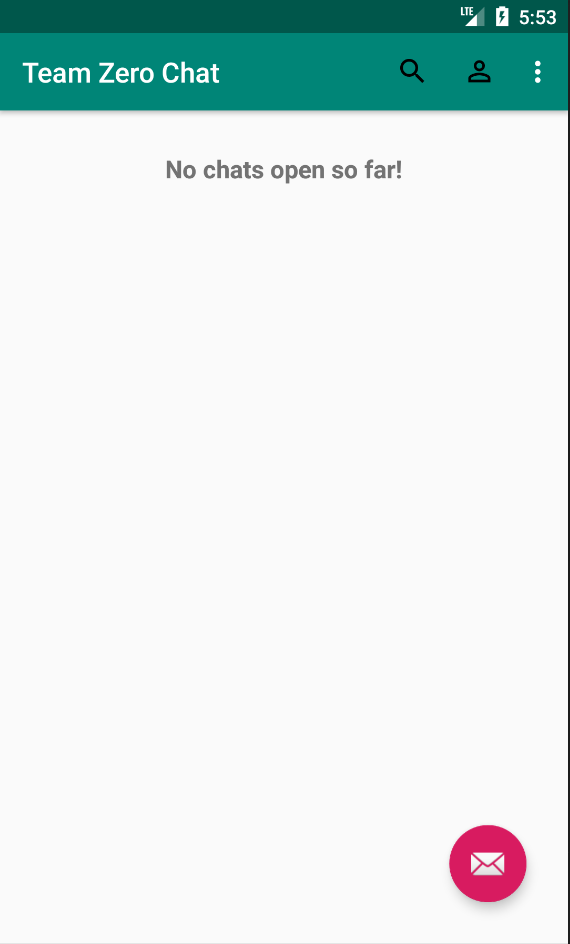
\includegraphics[width=.6\linewidth]{images/ChatList.png}
  \caption{ChatList Activity with no chats open}
  \label{chatListNoMessages}
\end{minipage}%
\begin{minipage}{.5\textwidth}
  \centering
  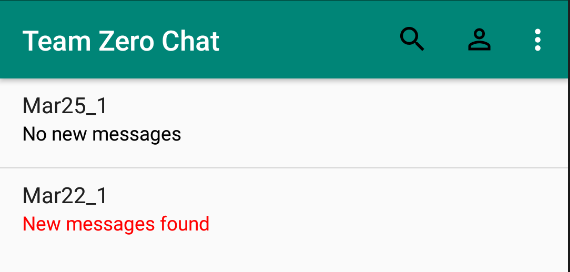
\includegraphics[width=.8\linewidth]{images/ChatListMessages.png}
  \caption{ChatList Activity with two chats open}
  \label{chatListWithMessages}
\end{minipage}
\end{figure}

% More specifically, the \verb|ListView| that contains the chats is made up of an \verb|ArrayAdapter| that has two separate lines (one for the username and one for the message status).

In order for a chat to NOT be considered as having unread messages, the user must click on the chat to view the content. This activity contains a \verb|runnable| action that checks \textbf{each 1 second} for new messages received through the WebSocket connection. Whenever there is a new message, it is put inside a variable that serves as a message queue containing the sender and messages. From that message queue, the sender is extracted and the algorithm analyses if the user currently logged in has already a chat open with the sender. If yes, it changes the status of the chat from "No new messages" to "New messages found" in red. If no, before changing the status, the new chat must be \textbf{appended to the chat list}. As part of this process, the client sends a \verb|getPublicKey| JSON request with the sender's username to find his/hers public key. Then the shared secret is calculated by using the \verb|generateSharedKey| method under the \verb|DHUtilities| class. It is then stored in the local database along with the sender's username, public key and a column named \verb|ChatBelongsTo| that must contain the receiver's username (i.e. you). The latter is \textbf{necessary} in order for the application to know which chats belong to which user logged onto the device. Without it, somebody can view view other users' chats and \textbf{access information that is not intended for him/her}.

From this activity, one can do any of the following actions:

1) Initiate a chat with a new user by clicking the red circle in the lower-right area of the screen

2) Select and open one of the user's chats that are already initiated (similar to what can be seen in figure \ref{chatListWithMessages})

3) Open up the settings in the upper-right side and select either to sign out, unregister the account, delete all the chats that are currently open or hide the chat history for this session only

Next up, we will explain the points above in the mentioned order.

\textbf{NewChat activity} (linked to the \verb|new_chat_layout.xml| front-end layout)

From this activity, the user can search for any other user that he wants to open a chat with. Upon entering this view, a sensible message appears on the screen announcing you of the steps needed to take in order to either \textbf{display all the users} (figure \ref{newChatDisplayAllUsers}) or just \textbf{search users by name} (figure \ref{newChatDisplaySelectUsers}). The resulted information is a list of users fetched from the server's database along with their \textbf{statuses} at the moment (offline/online). 

\begin{figure}[H]
\centering
\begin{minipage}{.5\textwidth}
  \centering
  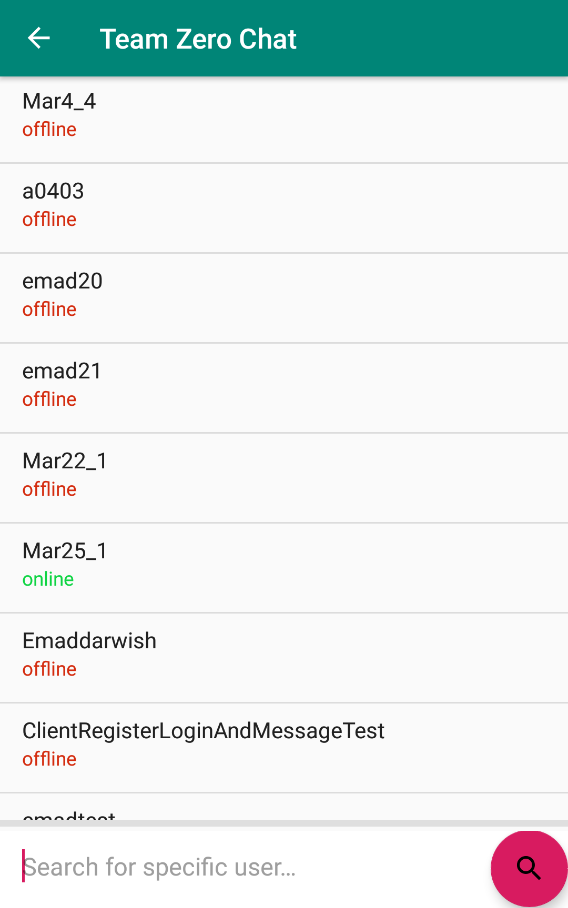
\includegraphics[width=.6\linewidth]{images/NewChatAllUsers.png}
  \caption{Display all users from the server}
  \label{newChatDisplayAllUsers}
\end{minipage}%
\begin{minipage}{.5\textwidth}
  \centering
  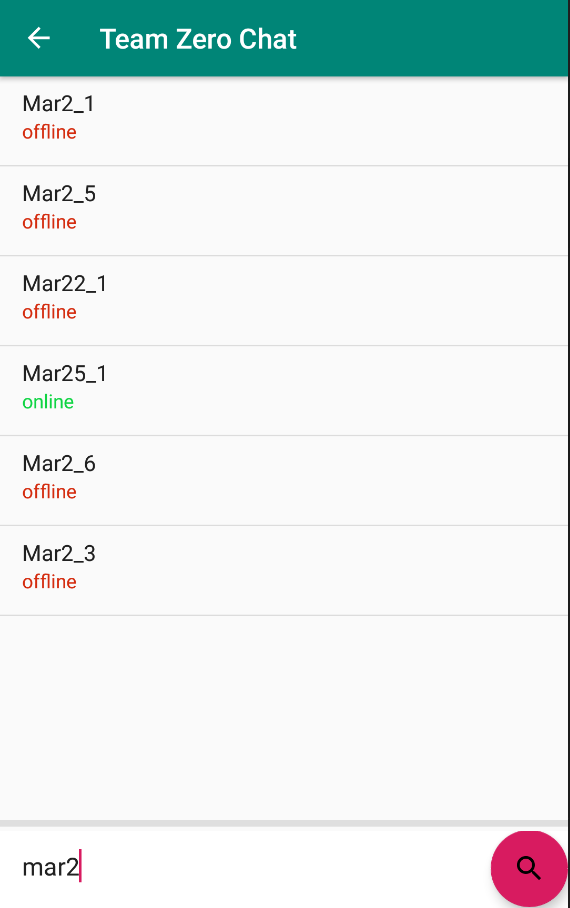
\includegraphics[width=.6\linewidth]{images/NewChatSelectUsers.png}
  \caption{Search for users}
  \label{newChatDisplaySelectUsers}
\end{minipage}
\end{figure}

If there are no registered users in the server's database or the server cannot find the username that you are searching for, our application tells you about the issue with a sensible message ("{\it{No contacts found on our database. Please try again.}}" or {\it{"No contact found with the requested name. Please try another name.}}").

From here on, the user can click on a person to initiate a chat with. The process that starts upon selection is similar to the process that takes place when receiving a message from a user that you do not have a chat with. The only difference is that because the \verb|GETALLCONTACTS| and \verb|SEARCHCONTACTS| JSON requests \textbf{already return the public keys} of the retrieved users, they are \textbf{directly stored into the local database} (no need to call \verb|GETPUBLICKEY| to fetch the public keys). After this, the view is returned to the chat list activity and the newly initiated chat can be seen in the list.

\textbf{Chat activity} (Linked to \verb|chat_layout.xml|)

The chat activity is the main point of communication between persons in the application. In here, the user can send/receive messages and view them. The figure \ref{chatExampleTwoUsers} shows an example chat between two users.

\begin{figure}[H]
 \centering
  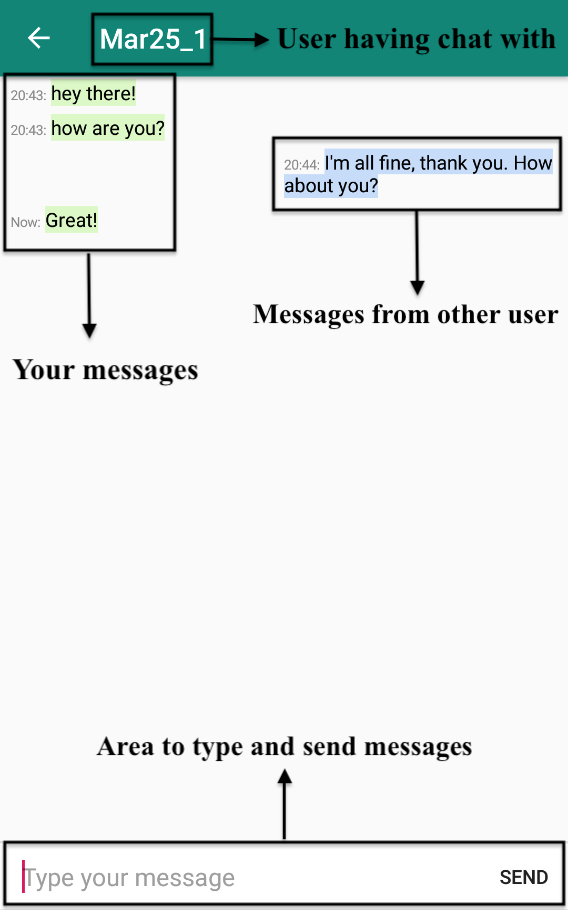
\includegraphics[width=0.3\textwidth]{images/Chat.png}
  \caption{Example chat between two users}
  \label{chatExampleTwoUsers}
\end{figure}

By default upon entering a chat, the application will execute a \verb|GETCHATHISTORY| JSON request to the server to retrieve the chat history for the \textbf{past 24 hours}. As seen on the left side of each message, there is a timestamp. \textbf{All the messages} that are currently sent or received in this session include a "Now:" in front of them. If the back button is clicked to return to the list of chats and then re-enter the same chat, the time in the format of \textbf{{\it{HH:MM}}} will appear instead (like in figure \ref{chatExampleTwoUsers}).

We have to mention that the messages received in this chat session are retrieved from a local message queue (\verb|messages| from the file \verb|UserDetails|). This queue is filled with messages received in real time by the WebSocket. If the sender of the message is this person that we are having a chat with, then just display his/her messages on screen and delete the content from the queue. This approach is much more efficient than periodically executing a \verb|GETCHATHISTORY| request from the server.

Thus, \verb|GETCHATHISTORY| is called \textbf{only once} to retrieve the history - When opening the chat session.

The messages are encrypted and decrypted using the shared secret computed from the other user's public key and your private key (step that happened either when you initiated a new chat \textbf{OR} when the other person initiated a new chat with you).

\textbf{Settings}

By clicking on the three dots sign (...) on the upper-right side of the screen with the chat lists, the user can access the settings. In there, he can do any of the following:

1) \textbf{Sign Out} - By signing out, the user is taken to the main login page upon which the app is launched on. The websocket connection is closed in order to signal the server that the user ended his online session.

2) \textbf{Unregister} - The app sends an \verb|UNREGISTER| JSON request to the server, then \textbf{deletes the user from the app's local database along with the chats owned by him}. After that, it closes the websocket connection and takes the user to the main login page.

\textbf{Important note:} before signing out or unregistering, we implemented in our code to \textbf{close the handler that checks every one second for the new messages}. We noticed that if this wouldn't have been implemented, then multiple instances of this handler were to be created when another user logs in. As they stack up, the application could've worked slower and slower until it became unresponsive and crashed.

3) \textbf{Delete All Chats} - By selecting this option, the user agrees to delete all his active chats so they no longer appear in his chat list. Deleting the chats removes all the previously stored information about them on this device, including the shared keys. However, it does \textbf{not} delete the messages that are stored on the server side.

4) \textbf{Hide Chat History} - This option allows the user to turn off (and back on) the retrieval of chat history for this current session of his online activity. By having this option on, the \verb|GETCHATHISTORY| JSON request to the server is \textbf{bypassed and not called} when entering a chat with somebody else.

\subsection{Other important implementation notes}

There is an interesting mention about the way we implemented the change of activities (i.e. going from one screen to another). We have used the \verb|setOnClickListener| method over the buttons instead of using \verb|android:onClick| at the XML level. For the latter, Android uses java reflection behind the scenes. Performance-wise, looking up a class via reflection is more computationally expensive than calling a method of the \verb|Button| class. We have used this approach throughout the whole application to avoid slowing down the performance.

We have disabled or changed the functionality of the native back button found on the lower left side of any Android device. This is important in order to \textbf{not allow the user to see sensitive information from other users that we're previously logged into the device}. This happens because the default Android button shows you \textbf{what the previous screen was}, and doesn't act like a “normal back button". For instance, if a user logged out and you click the default button, you can actually see the other user’s ChatList screen, exposing all of his chats to you. This was mitigated by bypassing this functionality with a custom one. On some activities like the launch login page or the chat list page, the default back button's functionality is disabled altogether and replaced with a sensible pop-up message. On the other activities, the button calls the \verb|onSupportNavigateUp| method. This method finishes the current activity (dismisses dialogs, closes searches etc.) and goes to the parent activity.

From a code perspective, an interesting note is that the \verb|GETCHATHISTORY|, \verb|GETALLCONTACTS| and \verb|SEARCHCONTACTS| JSON requests to the server can, sometimes, return only a single element. When returning more than one element, the JSON will contain an array delimited by square brackets ('[]'). In Java, for the array we can use a \verb|JSONArray| to fetch the data, but doing so onto a single object will result in a crash. For the latter, we have to use \verb|JSONObject| and have to cover the whole block of check into a try-catch (see lines 250-285 in \verb|Chat.java| file for example).

\subsection{WebSocket}

For the establishment of the persistent connection of the client to the server, we are using WebSocket version 1.3.0 (external library \verb|java-websocket-1.3.0|). This choice of version has been imposed across all of our platforms in order to ensure full compatibility between the clients and the server. We have also chosen this specific version because it is considered a stable and tested release, in order to increase the reliability of our system by decreasing the number of possible failures.

The websocket \textbf{is not serializable or parcelable}. In order to keep the same objects when changing activities, they need to be any of the above two. In this case, we cannot "pass" the connection from one activity to another. Because of this, we created a \textbf{handler class} (\verb|WebSocketHandler|)\textbf{with a static reference to the websocket} which we use to handle the connection and data exchange. With this approach, we can keep the connection alive during every activity in our application.

The \verb|onMessage| method adds the received messages received (either while online or offline upon login) to the message queue.

There are 2 different methods used to send messages to the server:

1) \verb|sendMessageAndWait| - Sends the message to the server and \textbf{awaits a response within a timeout period}. This method is used on requests to the server that require a response in order to proceed. A few examples include the login, registration, contact search etc. The timeout is set to 10 seconds, as we consider it a decent amount of time for a response. If the app does not receive a response within 10 seconds, it will display an appropriate message to the user telling him/her to try again.

2) \verb|sendMessage| - Sends the message to the server \textbf{without waiting for a response from it}. This method is used when sending text messages to other users, as the Android client does not need a response from the server and can continue it's actions.

\subsection{Local Database}

SQLite is at the core of our local database for the Android client. We can execute the CRUD actions directly using SQLite queries, but boilerplate code is mostly unavoidable this way. Because of this and the fact that Android Room efficiently converts tables into Java objects made the latter our primary choice.

There are multiple reasons for having a local database. One is that it stores information that does need to be passed to the server, like the private keys. Another is because of it's convenience in fetching data fast from the same device, as opposed to sending costly JSON requests to the server for each tiny information to be retrieved again (like the public keys of other users).

The figure \ref{androidLocalDatabase} displays the local database's schema.

\begin{figure}[H]
 \centering
  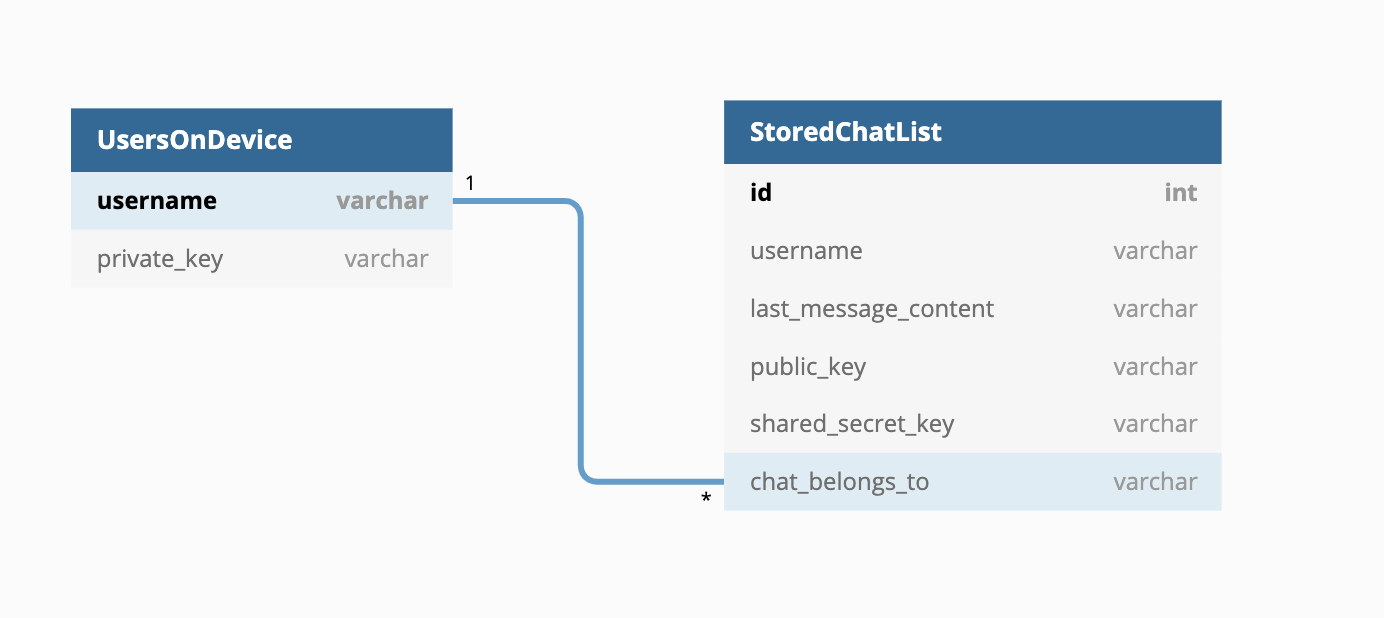
\includegraphics[width=0.8\textwidth]{images/AndroidLocalDatabase.png}
  \caption{Local Database Schema}
  \label{androidLocalDatabase}
\end{figure}

\textbf{UsersOnDevice} is the table that refers to the users registered on this device. It has the username for each user and his/her account's private key.

\textbf{StoredChatList} is the table which stores the chats for the users found in \textbf{UsersOnDevice}. \verb|id| is the primary key and it is auto-incremented after each insert. In here, the \verb|username| column refers to \textbf{the username with which} \verb|chat_belongs_to| \textbf{has a chat with}.

There is a one-to-many relation between the first table and the second one \\ (\verb|UsersOnDevice.username| $\rightarrow$ \verb|StoredChatList.chat_belongs_to|). This means that one username can have \textbf{zero, one or multiple chats} associated with his/her account.

Upon deletion of a user from this device, \textbf{all of his stored chats are deleted too}. From a technical perspective, this is accomplished by adding a {\it{cascade delete}} rule. The rule must run from \verb|UsersOnDevice| $\rightarrow$ \verb|StoredChatList| and not vice-versa. Thus, when removing username X from this device, it will automatically remove all the chats in \verb|StoredChatList| where \verb|chat_belongs_to| = X.

All of the operations that run on the local database are \textbf{completed as a background tasks}. The reason why is because each operation blocks the current thread on which it executes until it finishes. By running all the database operations on the main thread, the application will be greatly slowed down and the UI may remain locked for that period.

\subsection{Internal Tools}

\textbf{RegistrationValidator} is, as already explained in the chapter \ref{android-implementation}, the tool with which the login and registration fields are validated (figures \ref{tab:login_validations} and \ref{tab:registration_validations}). RFC5322 is the latest internet message format protocol that provides the formal definition of e-mail addresses \cite{RFC8322-e-mail}. We must mention the fact that our e-mail validation is \textbf{not fully RFC5322 compliant}. For instance, it does not accept e-mail addresses that contain single quotation marks (') like {\it{test'name@test.com}}. It also does not accept e-mail addresses that do not end with .[name], like {\it{admin@mailserver}}. However, it accepts most of the regularly used e-mail addresses and reject potentially malicious code like SQL injection. A full list of our tests will be displayed in the next chapter (\ref{android_unit_instrumented_testing}).

\textbf{JSONConstructor} is an internal tool that we've created to \textbf{easily construct JSONs} for requests sent to the server. It is a class which contains methods for each JSON request used in the distributed chat system. Let's consider the following example for the \verb|REGISTER| request (figure \ref{jsonConstructExample}).

\begin{figure}[H]
 \centering
  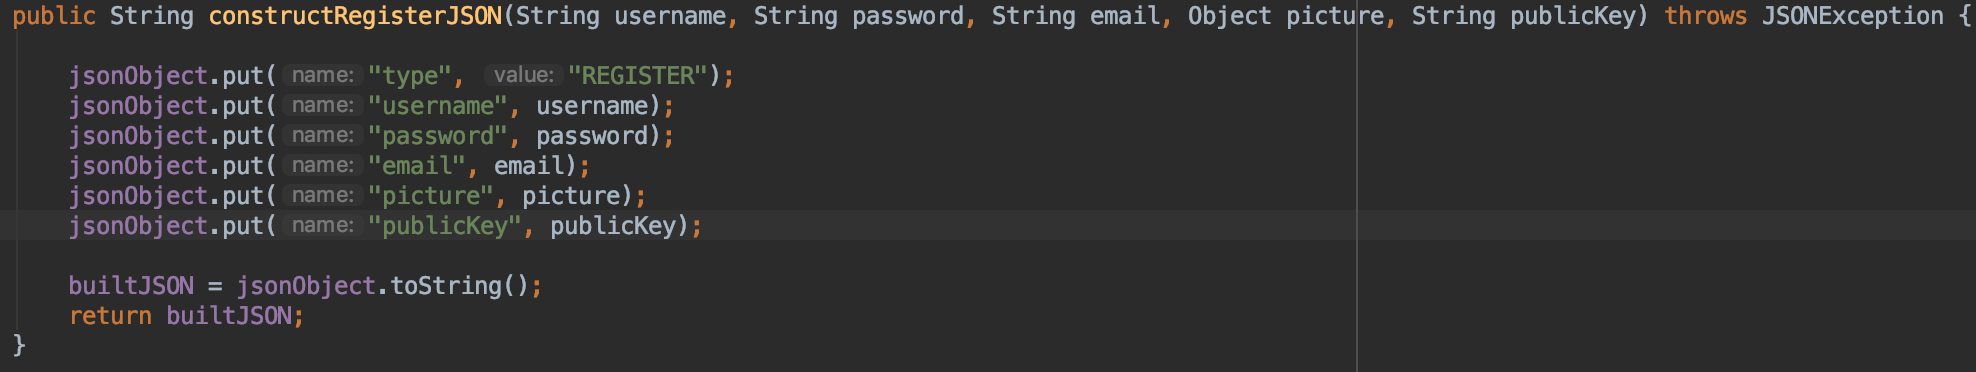
\includegraphics[width=0.9\textwidth]{images/JSONConstruct.png}
  \caption{Register JSON request construction}
  \label{jsonConstructExample}
\end{figure}

The method's arguments represent the values for each key. They are then used as 2nd arguments for the \verb|put| method of \verb|JSONObject| to form the JSON that will be sent to the server. We consider this an easier and more effective way to write code because the methods can be called in our activities whenever needed in a single line of code each.

\textbf{UserDetails / OtherUsersData} are files that store temporary information than can be used immediately. The first file contains fields related to the user currently logged in (like his username, who is he chatting with right now, his messages or is the history is hidden for this session). The latter serves as an intermediate way of passing information to the local database in an OOP fashion. For example, the information received from the server when the user initiates a new chat with another user, like the public key, is then stored temporary in an object of \verb|OtherUsersData|. It is then retrieved from there only when (and if) needed. This is a good thing to have because you may try to get a contact to chat with but then you change your mind, so the information must not get (yet) into the local database unless confirmed (by clicking the user you want to chat with from the list).

\textbf{Encryption utility files} include the following:

1) RFC5114KeyData - Contains the prime numbers P and Q in hexadecimal form that are used for the key generation with Diffie-Hellman.

2) DHUtilities - Contains the methods to generate public and private keys using prime numbers from \verb|RFC5114KeyData| file. It also contains the method that computes the shared secret between one public and one private key and 2 methods that transform a Base64 string into a public key. The latter is needed because the transmission to/from the server of public keys is done in Base64, so they need to be converted to the appropriate data type after.

3) AES256Cryptor - Is the filed that contains the encryption and decryption algorithm for our end to end protocol. It is done in AES CBC on 256 bits. More details about encryption in chapter \ref{encryption}.

\subsection{Unit Testing \& Instrumented Testing}
\label{android_unit_instrumented_testing}

We have executed several tests upon the mobile application to ensure the functionality and usability of the client. Other than the manual tests that have been executed every time after a feature was implemented, we have conducted a series of unit and instrumented tests on a few of the features.

The file \verb|RegistrationUnitTests.java| contains a series of \textbf{unit tests} specifically targeted at validations. They check for expected correct values, like a proper password with a decent strength (at least 1 uppercase, at least one special character etc.) and also for incorrect values that can have potentially harmful behaviour.

The following list includes a few examples of potentially harmful commands: \\
"\verb|"'OR 1=1--"@gmail.com|", "\verb|'OR 1=1--@gmail.com|", "\verb|'or 1=1-@gmail.com|", \\
"\verb|1'or'1'='1|", "\verb|' or 'a'='a|", "\verb|" or "a"="a|", "\verb|') or ('a'='a|", "\verb|") or ("a"="a|". They all can trigger an SQL injection attack to the server and it is the best to filter it out directly from the input, not only at server level.

In regards to the e-mail addresses, we have successfully tested the following types of formats in JUnit and they all work on our system: "\verb|lowercase@lc.com|", "\verb|UPPERCASE@UC.COM|", "\verb|eMaIL@EmAiL.cOm|", "\verb|test@email.co.uk|", "\verb|lowercase\_@UPPERCASE.COM|", \\ "\verb|email+100@email.com|", "\verb|email+100@e-mail.co.uk|".

% Made the Toasts that appear on registration page outside the methods (i.e. in Registration activity). Otherwise, unit tests wouldn't have been possible because getApplicationContext() used for Toast creation is not mocked

\textbf{JSONConstructionInstrumentedTests} includes the automated tests for the JSON request construction. It is used to generate multiple types of JSONs in various situations and compare its output to what is expected on the server end.

\subsection{Current Drawbacks}

Upon registration of a new user, a new set of public and private keys are generated using \verb|java.security.KeyPair|. The keys work for encryption and decryption between the same client (Android), but do not work when trying to chat with the web client. This happens because the generated keys in Base64 in \verb|java.security| (Android client) are of different size than the keys generated in Base64 in \verb|CryptoJS| (web client). Because there are discrepancies between the clients in the way the keys are generated, we have decided as a trade-off to use a sample set of keys generated using the web client's CryptoJS library. More information about the encryption in the chapter \ref{encryption}.

Right now, the same user can be added more than once in the chat list. This does not disrupt the application in the way it functions, but you can see multiple chats with user A if you choose to initiate more than one chat with A (and they all contain the same chat history). This can be mitigated by querying the local database in order to check if that user already exists or not in your chat list.

Every time a user enters a chat, it retrieves the chat history by sending a JSON request to the server. It is not the most efficient approach because it's an expensive operation in regards to time passed. It is better to store the messages in the local database.

As backwards compatibility comes to mind, clients that did not register on this specific Android device cannot chat. This happens because after logging in and either receiving messages or initiating a new chat, the app tries to retrieve the private key of the user. Because the server does not get/send private keys and the mobile devices does not have the private key, it will result in a crash.

% There is a small chance that at login, when the user receives messages that were sent to him while being offline, those messages would appear in the websocket queue before the LOGIN response from the server appears. This would not make the application crash and nor the login process fail, but it will make it much slower. Particularly, it will freeze for 10 seconds. This is the time it takes for the TimeoutException of the concurrent thread to be thrown. --> This was managed to be partially solved by adding a small delay when sending messages to the client that were received while being offline. The delay would not add up for the server and does not pose a scalability problem because it works on different threads, so basically just one thread on the server would be affected by the small delay (which is hard-coded to 10 ms).

\subsection{Further Improvements}

The status of the internet connection can be monitored by using different methods found in \verb|android.net.ConnectivityManager|. It can be a good idea to send broadcast intents when the network connectivity is lost so the user is notified of the problem (and remain on a buffering screen so that the user comprehends that the application is doing background work while reconnecting to the internet). If the user wants to close the application, it's also possible to store the ID of the last screen onto which the user was interacting, in the local database. This is possible because the local database can be accessed with or without the internet connection. After the app is opened again and the internet connection is live, it can resume from the stored checkpoint. The permissions that are being used for these actions are \verb|ACCESS_NETWORK_STATE| and \verb|ACCESS_WIFI_STATE| (the latter is useful for accessing the \verb|android.net.wifi.WifiManager| that manages all aspects of the WiFi connectivity in particular). They are already inserted in the Manifest file of the application and require using the \verb|getActiveNetworkInfo| method over the \verb|ConnectivityManager| to check the connection status.

Adding the possibility to retrieve the chat history for any amount of time the user wants to. It can take the form of a new element in the drop-down list of the settings named "Chat History Time" and then the user can select from a spinner the number of hours/days to retrieve the history from.

In regards to the chat history hide mode, if user A turns off the chat history and logs back in, it will automatically be on again. A possibly better implementation would be to register in the local database the choices made by this particular user and know it for further usage (i.e. remember his choice when he logs back in).

The "remember login credentials" check from the login page does not have the functionality implemented yet. It can be implemented by adding another column to the \verb|UsersOnDevice| table to store if the check is on or off. If it is on, then it can automatically login back into the account until the user explicitly signs out and the flag is turned to {\it{false}}.